\section{Environnement Professionnel}
\subsection{L'entreprise}
\subsubsection{Mission-Vision}
De la démocratisation du BPM à la transformation numérique en profondeur de l'entreprise, nous sommes à la pointe d'une révolution professionnelle depuis que notre entreprise a vu le jour.
Le succès de nos clients est notre succès, et tout le monde chez Bonitasoft est un contributeur, chaque jour.
\cite{Bonitasoft2017BONITA1}

\subsection{Un peu d'Histoire}
Bonitasoft est un éditeur de logiciel open source créé en 2001. Il a commencé comme
Bonita BPM dans l'Institut National de Recherche en Informatique et en
Automatique (INRIA) puis transféré au Groupe Bull.
En 2009, Miguel Valdés Faura rejoint Charles Souillard et Rodrigue Le Gall pour
fonder Bonitasoft.
En 2011, après une série de levée de fonds, Bonitasoft a pu commercialiser son
produit Bonita à l'international et le premier bureau de Bonitasoft est ouvert
aux Etats-Unis.\cite{wikipedia_2018}



\subsection{Organisation}
Bonitasoft a quatre bureaux principaux, aux États-Unis, à San Francisco et à New York,
en France à Paris et à Grenoble.
Les activités sont organisée et divisée en 5 different services:


\begin{center}
  \smartdiagramset{bubble node size=4cm, bubble center node size=6cm}
  \smartdiagram[bubble diagram]{Bonitasoft,
  IT,Service Professionnel,
  R\&D, Support, Succès du Client}
\end{center}


\subsubsection{IT}
Le département de l'IT est le gardian principal de tout le tâches IT commun comme:
\begin{itemize}
  \item La gestion des environnements virtuels. (cloud ou serveur physique).
  \item La gestion de l'automatisation de processus de CI interne.
  \item La gestion des licences des applications payent (OS, applications).
  \item La gestion des appareils, périphériques, les ordinateurs portables,
  \item L'architectures, méthodologies et règles régissant l'utilisation et le stockage des données.
  \item L'administration de systèmes: la configuration, gestion, entretien et dépanne des environnement
  informatique multi-utilisateur (cloud ou physique).
  \item  La gestion ou l'aide aux autres département avec la culture et pratiques DevOps.
\end{itemize}

Aussi, l'équipe d'IT de Bonitasoft gère d'autres projets comme:
\begin{itemize}
  \item Salesforce: depuis la création des use cases jusqu'à la mise en production en garantissant la gouvernance du système avec une approche DevOps.
  \item BCD: c'est une solution fournit pour utiliser les bonnes pratiques DevOps pour la livraison continue (CI) d'une application Bonita.
\end{itemize}

L'équipe est composée de quatre personnes, dont l'une est moi.

\begin{figure}[h]
  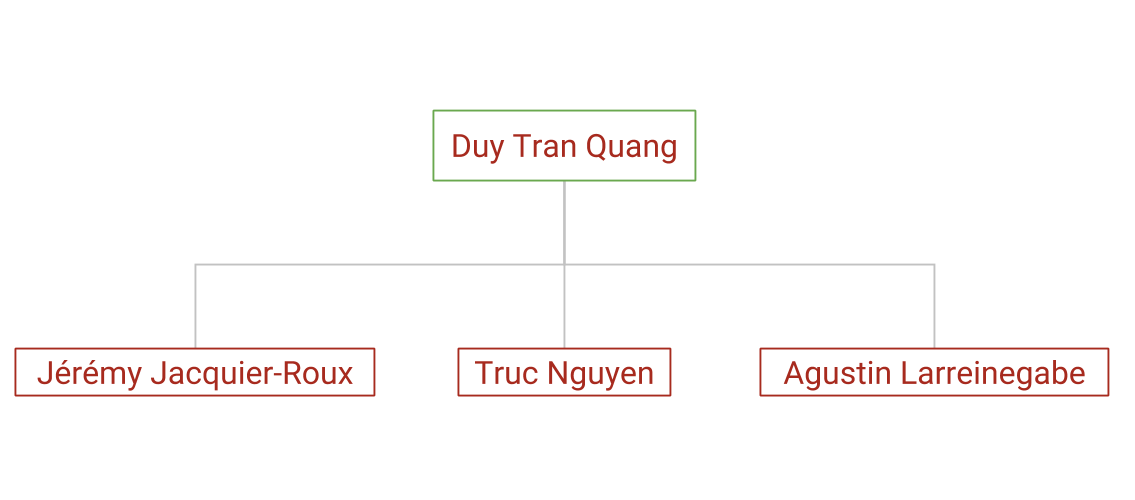
\includegraphics[width=\textwidth,keepaspectratio]{it_team.png}
   \caption{Organigramme.}
   \label{figure:organigrame}
\end{figure}

\subsubsection{R\&D}
Il est le plus grand département et son travail principal est le développement de la plate-forme Bonitasoft.
Il est divisé par équipes de travail ou projets:
\begin{itemize}
  \item Back-end
  \item Front-end
  \item BICI, c'est une application autonome connectée au moteur de Bonita qui permet d'analyser l'exécution
   des processus et prévoir et améliorer l'efficacité de l'équipe.
\end{itemize}

\subsubsection{Customer Success (CS)}
Le département gère la relation entre Bonitasoft et ses clients. L'objectif de la réussite du client est de rendre le client le plus performant possible, ce qui, à son tour, améliore la valeur à vie du client pour l'entreprise.
Cette fonction est la plus couramment utilisée dans le monde du logiciel et la plus répandue parmi les sociétés de services. Parce que le succès du client est un domaine naissant, son alignement organisationnel et ses activités sont toujours en évolution.

\subsubsection{Support}
Ce département est en charge de traiter et de diriger les différentes questions et problématiques du client.
Chaque problème ou bogue est chargé dans l'outil Jira et traité par le département R\&D ou l'IT.
Chaque ticket chargé a une priorité et il est résolu par ordre de priorité.

\subsubsection{Service Professionnel}
C'est une équipe d'experts qui offre de la valeur pour le succès du client en suivant les projets depuis le début avec la meilleure expérience-utilisateur possible.

